\chapter{Theoretical Background}
\label{chap:02}
\paragraph{}
Cell-cell signalling is the process by which cells communicate with each other within the body. This communication can occur between cells that are next-door neighbours or between cells that are far apart. There are several different types of cell-cell signalling, including paracrine signalling, autocrine signalling, endocrine signalling, and synaptic signalling. In terms of numerical methods, these are mathematical techniques that are used to model and simulate complex systems. Numerical methods can be used to study a wide range of problems, including those in physics, engineering, and biology. In the context of cell-cell signalling, numerical methods can be used to model the dynamics of signalling pathways, predict the behaviour of cells in response to different signals, and design new drugs that target specific signalling pathways. These methods can include techniques such as differential equations, linear algebra, and optimization. So in this chapter theoretical background of cancer cell-cell signalling and its mathematical background will be discussed. 

\subsection{Biological introduction of cell signalling}
\paragraph{}
Cells develop and proliferate out of control in cancer, which is a disease. Cancer cells create a number of distinctive modifications in their cell signalling pathways as the tumour grows \cite{peng2017lncrna}. These modifications include the ability to proliferate without exogenous growth-promoting or growth-inhibitory signals, invade nearby tissues and metastasize to distant sites, elicit an angiogenic response, and evade cell proliferation-limiting mechanisms like apoptosis and senescence \cite{crosas2022rho}. Understanding these changes in cell signalling pathways and how they affect the onset and spread of cancer is the primary goal of research in cancer biology and cell signalling. For the purpose of enhancing precision medicine treatments for hormone-related and genitourinary cancers, this includes researching tumour evolution, drug sensitization, and oncogene network modifications in patients. 

Cytokine receptors and receptor tyrosine kinases (RTKs) are proteins that start cell signalling cascades \cite{kazi2014socs}. The intracellular section of RTKs has a tyrosine kinase domain that enables them to phosphorylate other proteins, initiating a signalling cascade. On the other hand, in order to start signalling, cytokine receptors need to join forces with other intracellular proteins known as Janus kinases (JAKs) \cite{gadina2013janus}. A cytokine receptor that is not linked to a JAK molecule lacks the kinase activity that the JAK molecules have. Both varieties of receptors start the intracellular signalling pathways when they attach to particular substances in the extracellular environment known as ligands. The sort of ligands that these two types of receptors bind—RTKs mainly bind to growth factors, whereas Cytokine receptors primarily bind to cytokines—is the fundamental distinction between them \cite{tamiya2011suppressors}.

 \begin{figure}[hbt!]
	\centering
	\begin{framed}
	\includegraphics[width=0.8\textwidth]{Figures/a.JPG}
		\end{framed}
	\caption{Diagram of the JAK/STAT signalling pathway, initiated by cytokine molecules, taken from \cite{haan2006jaks}. The red stars attached to a species indicate that the species is phosphorylated.}
	\label{fig:6}
\end{figure}

\subsection{Genetic alterations in signalling pathways}
\paragraph{}

Modifications in the genes that regulate cellular processes like cell division and cell death are referred to as genetic changes in signalling pathways\cite{strasser2000apoptosis}. These changes can be brought about by gene fusions, copy-number changes, mutations, and mRNA expression \cite{kang2016integrated}. These modifications can result in the unchecked cell growth and proliferation that characterise cancer. Melanoma, where mutations in the RAS signalling cascade are almost universally present, is one example of genetic changes in signalling pathways. Although RAS itself is rarely mutated in melanoma, RAS is downstream from BRAF on the protein kinase B/Akt pathway and PTEN on the mitogen-activated protein kinase pathway. These genes are frequently altered in melanomas; BRAF is the most frequently mutated gene in melanomas \cite{haluska2006genetic}. Understanding the genetic alterations in signaling pathways is an essential aspect of cancer research and treatment, as these alterations can be targeted with drugs and therapies to limit the growth and spread of cancer cells. 



\subsection{RORs (Receptor Tyrosine Kinases) in cancer and its downstream signalling}
\paragraph{}

Receptor Tyrosine Kinases (RTKs) play a critical role in cancer by initiating cell signalling pathways \cite{butti2018receptor}. RORs (Receptors of RAS-related Orphans) are a subfamily of RTKs that have been shown to impact cancer significantly \cite{kamrani2019therapeutic}. RORs are a group of receptors that are activated by ligands and are involved in cell growth, differentiation and the formation of blood vessels. In cancer, RORs are often dysregulated, and this leads to overactive or abnormal signalling within and among these pathways that may contribute to the survival of cancer stem cells (CSCs). The dysregulation of RORs can lead to the formation of new blood vessels, the ability of cancer cells to migrate and invade other tissues, and the resistance to chemotherapy and radiation therapy \cite{pan2016emerging, mahmoudian2021interaction}. To understand it better, refer to Figure \ref{fig:2}, which will help you understand the process more precisely and engagingly. This image will provide a visual representation of how RORs work in cancer and how they contribute to the development of cancer. Additionally, it will also provide a better understanding of the downstream signalling pathways that are activated by RORs and how they lead to the formation of cancer.


 \begin{figure}[hbt!]
	\centering
	\begin{framed}
	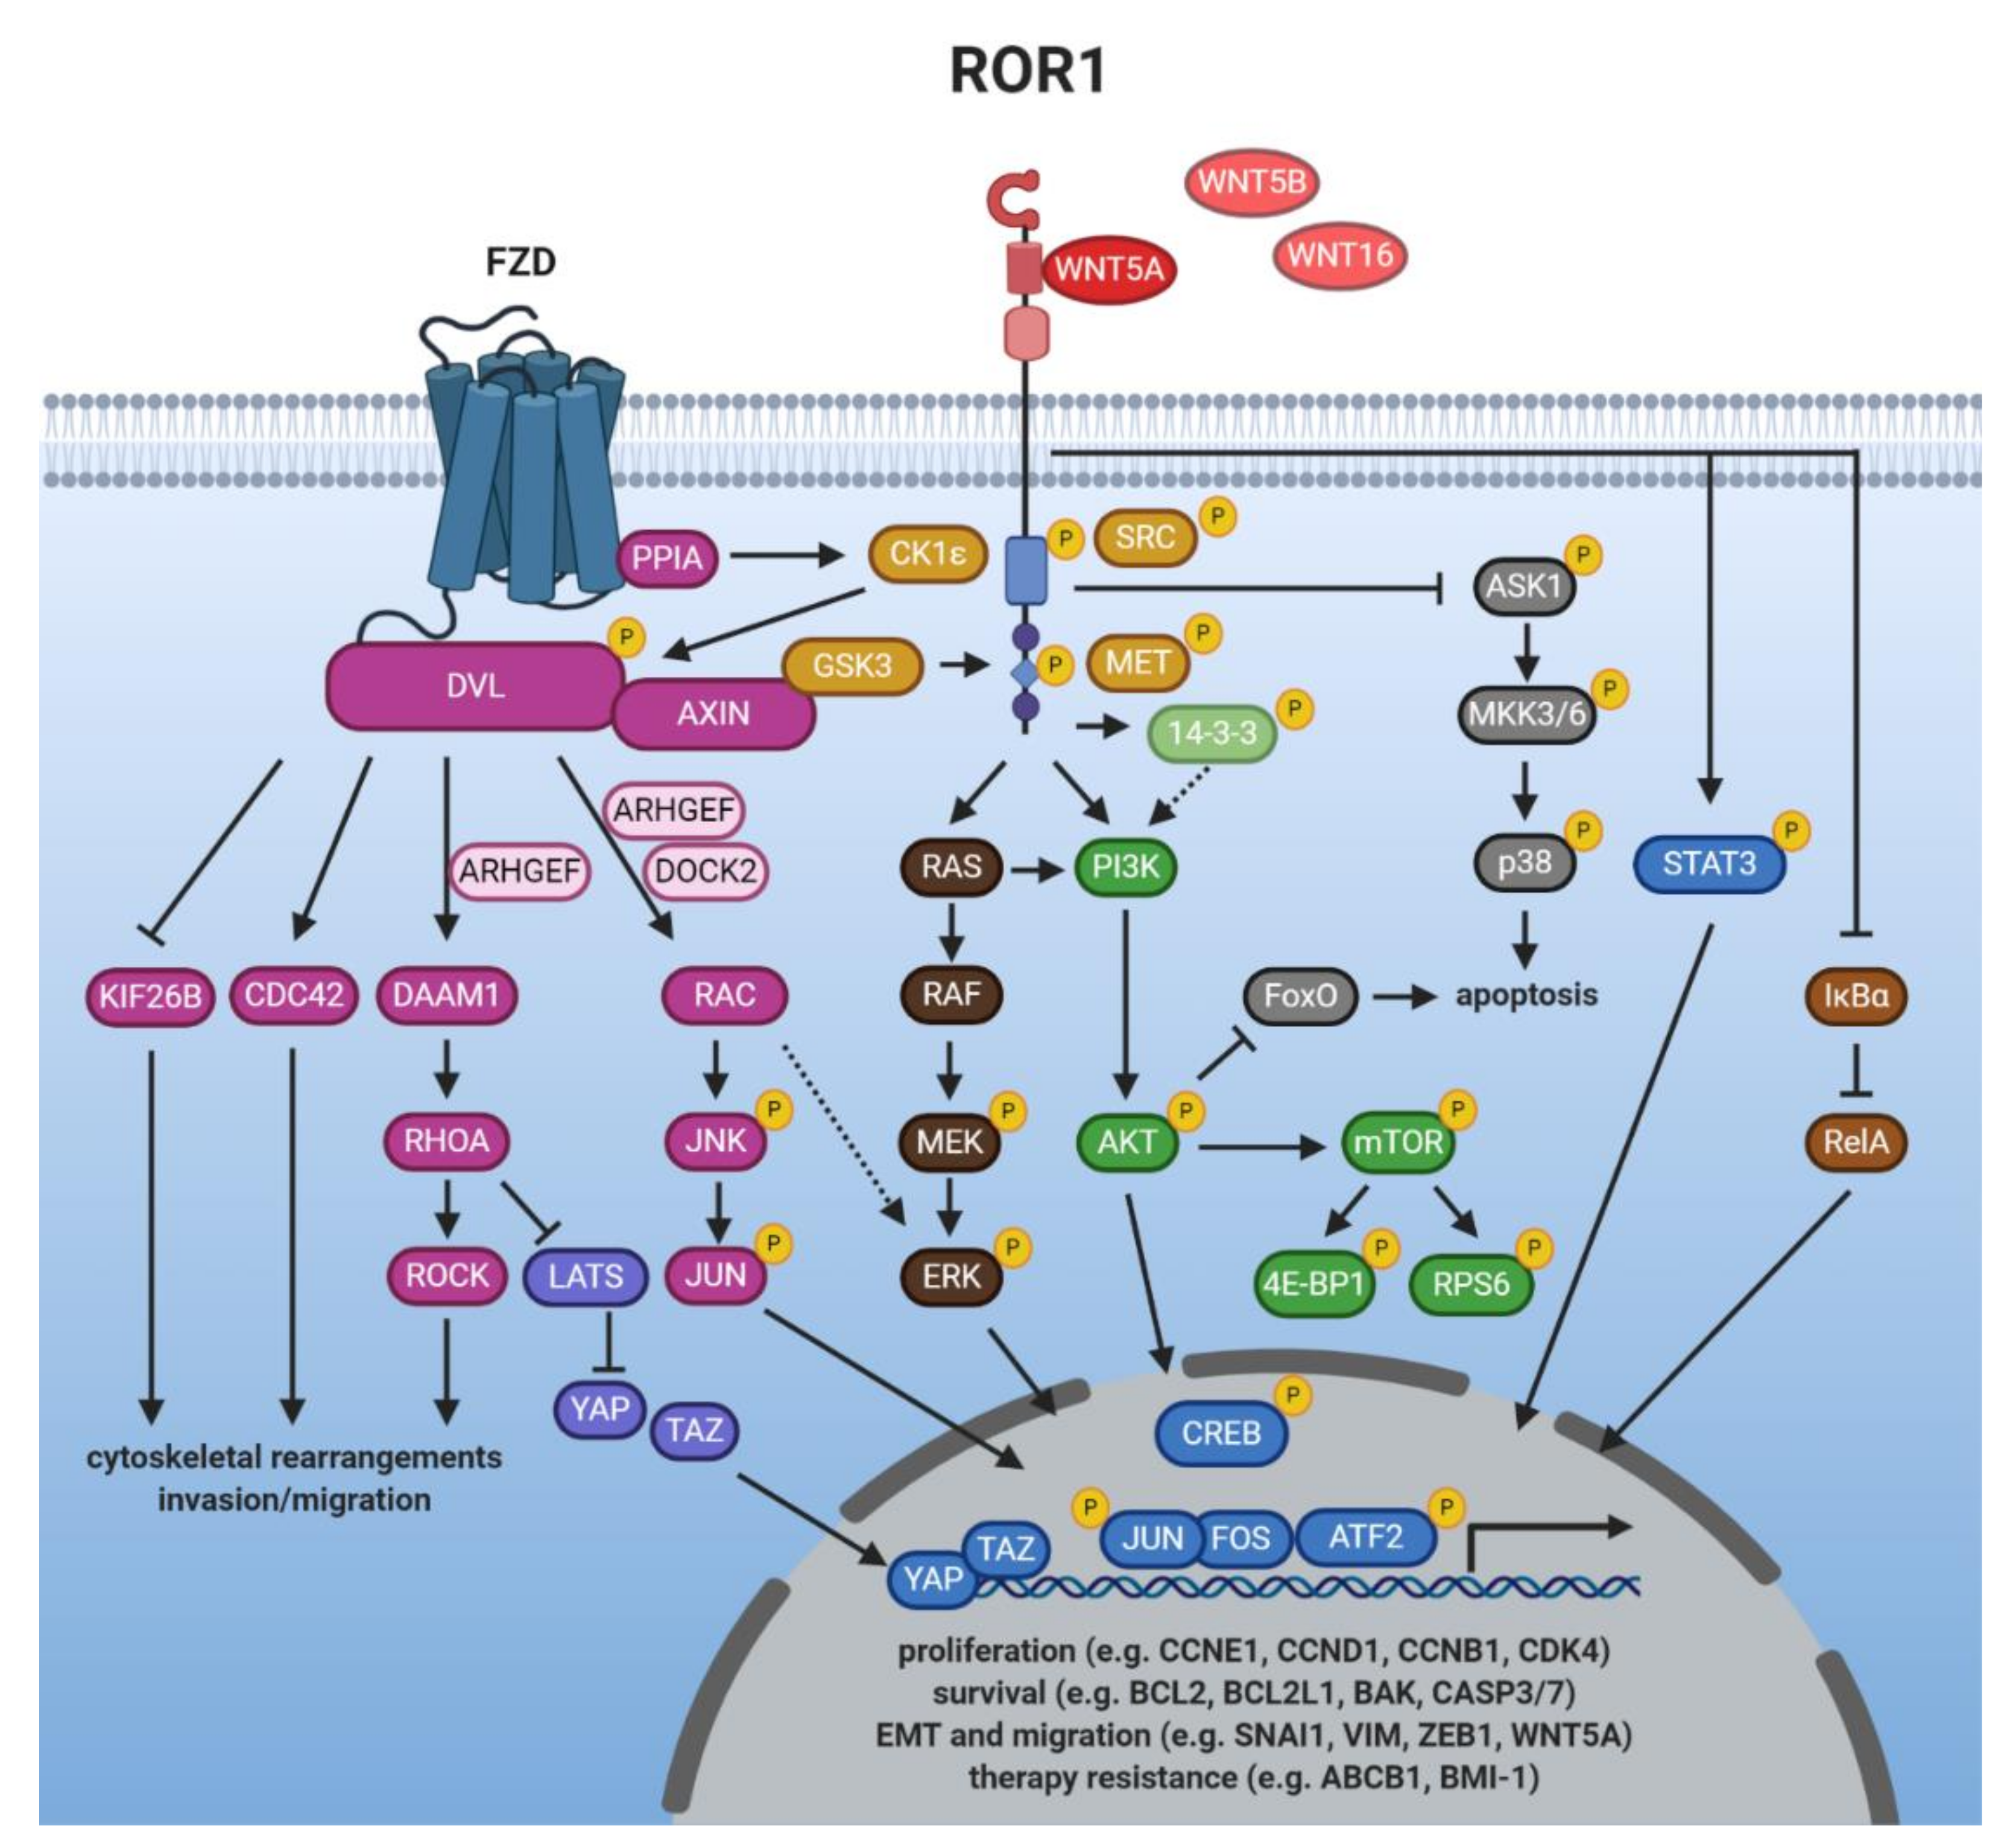
\includegraphics[width=0.8\textwidth]{Figures/b.png}
		\end{framed}
	\caption{ROR1 signaling. WNT/ROR1 signalling is induced by the binding of a non-canonical WNT ligand, which triggers the formation of a complex between ROR1 and ROR2, or ROR1 and a FZD receptor, respectively \cite{menck2021wnt}. }
	\label{fig:2}
\end{figure}

\subsection{The current state of knowledge about the signalling pathways involved in cancer and the challenges in understanding these pathways.}
\paragraph{}

The aberrant cell proliferation that characterises cancer is a complex disease. Numerous signalling pathways have been linked to the development and spread of cancer, but the precise processes by which these pathways cause the disease are still poorly understood. The RAS signalling cascade, which is frequently changed in a range of tumour forms, is one of the important signalling pathways in cancer \cite{maruta1994regulation}. A mutation in a member of the RAS family of proteins, which is involved in cell growth and differentiation, can result in uncontrolled cell proliferation and the emergence of cancer. Other signalling pathways like PI3K-Akt, Wnt, and Notch have also been discovered to have a role in the development and spread of cancer \cite{rizzatti2005gene, lombardi2013solar}.

The complexity of the interactions between many signalling channels presents one of the difficulties in understanding these pathways. It is challenging to pinpoint the precise function of any one process in the disease, for instance, because alterations in one pathway can affect the activity of other pathways. The fact that numerous alternative pathways can activate the same pathway further complicates our knowledge of the disease. Cancer is a diverse illness, and various cancer forms might have various genetic and molecular alterations. Consequently, it is challenging to create targeted medicines that are efficient in treating all cancer types \cite{meng2017identification, hansen2015gut}. 

In conclusion, there is still much to learn about the precise methods by which the signalling pathways involved in cancer contribute to the disease. These pathways are intricate and multifaceted. Further study is required to comprehend these pathways better and create cancer medicines that work.

\subsection{Numerical analysis}
\label{Num}

\paragraph{}
Numerical analysis is a branch of mathematics that teaches computer methods for studying and solving mathematical issues \cite{burden2015numerical}. In this section, we look at numerical approaches for solving the most frequent mathematical problems and analyse the errors that can occur while using these methods. Because practically all computation is now done on digital computers, we also explore the consequences of numerical method implementation.

The investigation of errors is vital to numerical analysis. Most numerical approaches produce responses that are simply approximations of the intended genuine solution, and it is critical to understand the associated error and, if feasible, estimate or constrain it \cite{heydari2016theoretical}. This study looks at the numerous errors that can occur in a situation. The representation of numbers in computers, as well as the mistake in computer arithmetic, are investigated \cite{cui2018numerical}. The general results on the propagation of errors in calculations are presented, along with a detailed examination of errors in summing processes. Especially in this study, we will consider the Runge Kutta fourth-order (RK4) method \cite{islam2015comparative}. 

\subsubsection{Runge Kutta fourth order method}
\label{RK}

\paragraph{}

The fourth-order Runge-Kutta technique explains the lengthy computation of numerous unknowns, and the comprehensive step-by-step derivation and analysis can be found in many publications \cite{tan2012general, mehdi2017using}. Because of the method's importance in mathematics and applied science/engineering. By reviewing specific, possibly well-known papers, we simplify and minimise the complexity of their derivation and analysis by proposing a step-by-step derivation of the method.

In 1901, two German men, Carl Runge (1856-1927) and Martin Kutta (1867-1944), devised the Runge-Kutta Method \cite{tobies2012iris}. Carl Runge created numerical methods for solving differential equations that evolved from his research on atomic spectra. These numerical techniques are still in use today. He employed so much mathematics in his studies that physicists mistook him for a mathematician, and he employed so much physics that mathematicians mistook him for a physicist. His name is now synonymous with the Runge-Kutta methods for numerically solving differential equations. Kutta, another German applied mathematician, is well recognised for his contribution to the Kutta-Joukowski theory of airfoil lift in aerodynamics, which is based on differential equations \cite{trefethen2015invented}. 


\subsubsection{Runge-Kutta 4th order method to solve differential equation}

Given the following inputs \cite{rungekutta_2023_webpage}. 

\begin{itemize}
    \item An ordinary differential equation that expresses the value of $dy/dt$ in terms of $t$ and $y$.
    \item Initial value of $y$, i.e., $y(0)$. 
\end{itemize}

\begin{equation}
    {{dy(t)} \over {dt}} = y'(t) = f(y(t),t), \quad \quad {\rm{with\;}} y(t_0)=y_0
\end{equation}

The evolution of the Fourth Order Runge-Kutta method closely parallels that of the second Order and will not be discussed in depth here. Like the second-order method, the fourth-order method has several variations that all employ four estimates of the slope. To determine the slope at some time t0 (assuming we just have an approximation to $y(t_0)$ (which we call $y^*(t_0)$), we will utilise the following slope approximations.

 \begin{figure}[hbt!]
	\centering
	\begin{framed}
	\includegraphics[width=0.7\textwidth]{Figures/F.JPG}
		\end{framed}
	\caption{Slopes used by the classical Runge-Kutta method \cite{hossain2017comparative}.}
	\label{fig:6}
\end{figure}

\newpage

\begin{equation}
    {k_1} = f({y^*}({t_0}),{t_0})
\end{equation}

\begin{equation}
    {k_2} = f\left( {{y^*}({t_0}) + {k_1}{h \over 2},{t_0} + {h \over 2}} \right)
\end{equation}

\begin{equation}
     {k_3} = f\left( {{y^*}({t_0}) + {k_2}{h \over 2},{t_0} + {h \over 2}} \right) 
\end{equation}

\begin{equation}
    {k_4} = f\left( {{y^*}({t_0}) + {k_3}h,{t_0} + h} \right)
\end{equation}

Each one of these slope estimates can be directly explained. 

\begin{itemize}
    \item $k_1$ is the slope at the beginning of the time step (this is the same as $k_1$ in the first and second order methods).
    
\item If we use the slope $k_1$ to step halfway through the time step, then $k_2$ is an estimate of the slope at the midpoint. This is the same as the slope $k_2$, from the second-order midpoint method. This slope proved to be more accurate than $k_1$ for making new approximations for y(t).

\item If we use the slope $k_2$ to step halfway through the time step, then $k_3$ is another estimate of the slope at the midpoint.

\item Finally, we use the slope, $k_3$, to step all the way across the time step$(t_0, t_0+h)$, and $k_4$ is an estimate of the slope at the endpoint. 
\end{itemize}

We then use a weighted sum of these slopes to get our final estimate of $y^*(t_0+h)$.

\begin{equation}
    {y^*}({t_0} + h) = {y^*}({t_0}) + {{{k_1} + 2{k_2} + 2{k_3} + {k_4}} \over 6}h 
\end{equation}



\begin{equation}
   {y^*}({t_0} + h) = {y^*}({t_0}) + \left( {{1 \over 6}{k_1} + {1 \over 3}{k_2} + {1 \over 3}{k_3} + {1 \over 6}{k_4}} \right)h
\end{equation}

\begin{equation}
   {y^*}({t_0} + h) =  {y^*}({t_0}) + mh
\end{equation}

 {\rm{where\;}}m{\rm{\;is\;a\;weighted\;average\; slope\; approximation.}}

The approach is comparable to the second-order endpoint method \cite{dontchev2000second}, which employed an equal weighting of the slopes at the start and end of the interval. The weighting of the midpoint slopes ($k_2$ and $k_3$) is larger than that of the endpoint slopes ($k_1$ and $k_4$) in this case because we expect these to be a better estimate of the slope while travelling from $y^*(t_0)$ to $y^*(t_0+h)$.

\newpage
 \subsubsection{Euler's numerical method}
 \paragraph{}

Euler's method is a numerical method used to approximate solutions to first-order ordinary differential equations (ODEs) called initial value problems. It is named after the Swiss mathematician Leonhard Paul Euler (1707-1783) \cite{biswas2013discussion, zondervan1998review}. The basic idea behind Euler's method is to approximate the solution of an ODE by constructing tangents to the solution curve at discrete points using a simple formula. The method is based on the assumption that the tangent line to the solution curve of the ODE at a given point approximates the solution curve over a small interval. Euler's method uses the simple formula, $y(x+h) = y(x) + hf(x,y)$ to construct the tangent at the point x and obtain the value of y(x+h), whose slope is $f(x,y)$ \cite{mazandarani2013modified}. This method can be used to approximate the solution of a first-order ODE by creating a sequence of short-line segments at steps of $h$. However, Euler's method is considered crude and not widely used in practice due to its low accuracy. 

\subsubsection{Euler's method to solve differential equation}
\paragraph{}

Euler's method is a first-order numerical procedure for solving ordinary differential equations (ODEs) with a given initial value. 

 \begin{figure}[hbt!]
	\centering
	\begin{framed}
	\includegraphics[width=0.65\textwidth]{Figures/euler.PNG}
		\end{framed}
	\caption{Slopes used by the Euler's method \cite{freecodecamp.org_2021}.}
	\label{fig:6}
\end{figure}


The general initial value problem methodology is given by the equation: 

\begin{equation}
    x_n = x_0 + nh
\end{equation}
\begin{equation}
    y_n = y_{n-1} + hf(x_{n-1}, y_{n-1})
\end{equation}

where $h$ represents the step size and $n$ is an integer, starting with 1. The number of steps taken is counted by the variable $n$. This method is based on the assumption that the tangent line to the integral curve of the ODE at $(x_n, y(x_n))$ approximates the integral curve over the interval $[x_n, x_{n + 1}]$. The formula used in Euler's method is:

\begin{equation}
    y(x+h) = y(x) + hf(x,y)
\end{equation}

where $f(x,y)$ is the derivative of y with respect to $x$, and h is the step size. This formula can be used to construct the tangent at the point x and obtain the value of $y(x+h)$ whose slope is $f(x,y)$. Euler's method can approximate the curve of the solution by the tangent in each interval (by a sequence of short line segments) with steps of $h$. 






